% =====================================================================
% paper.tex — UC3M MSc CSS final paper, Spring 2026
% Author: Abdullah Tadmuri (100502844)
% Course: Social and Ethical Issues of Big Data & AI
% Deadline: Friday, 22 May 2026
% Target length: 2,500–3,500 words; this draft targets 3,200.
% =====================================================================

\documentclass[12pt]{article}

% --- Page geometry: UC3M-style A4, 2.5cm vertical, 3cm horizontal ---
\usepackage[a4paper, vmargin=2.5cm, hmargin=3cm, headheight=14pt, headsep=12pt]{geometry}

% --- Fonts: Times New Roman 12pt ---
\usepackage{mathptmx}
\usepackage[T1]{fontenc}
\usepackage[utf8]{inputenc}
\usepackage[english]{babel}

% --- Math ---
\usepackage{amsmath}
\usepackage{amssymb}

% --- Spacing: 1.5 line spacing ---
\usepackage{setspace}
\onehalfspacing

% --- Typography quality ---
\usepackage{microtype}

% --- UC3M brand colour ---
\usepackage[table]{xcolor}
\definecolor{azulUC3M}{RGB}{0,0,102}

% --- Figures, tables, captions (UC3M social-sciences style) ---
\usepackage{graphicx}
\graphicspath{{figures/}}
\usepackage{float}
\usepackage{booktabs}
\usepackage{multirow}
\usepackage{caption}
% Caption label in UC3M blue + small caps + bold ("Figure 1." stands out)
\DeclareCaptionLabelFormat{uc3m}{\textcolor{azulUC3M}{\textbf{\textsc{#1 #2}}}}
\captionsetup{
  labelformat=uc3m,
  labelsep=period,
  font=small,
  justification=raggedright,
  singlelinecheck=false,
  skip=6pt
}

% --- Section title formatting (UC3M-style: bold, slightly larger, blue accents) ---
\usepackage{titlesec}
\titleformat{\section}
  {\Large\bfseries\color{azulUC3M}}
  {\thesection.}
  {0.5em}
  {}
\titleformat{\subsection}
  {\large\bfseries\color{azulUC3M}}
  {\thesubsection.}
  {0.5em}
  {}
\titlespacing*{\section}{0pt}{18pt}{8pt}
\titlespacing*{\subsection}{0pt}{10pt}{4pt}

% Two-line section title macro: primary name on line 1, descriptive subtitle on line 2.
% Optional short form for TOC keeps "Main: Sub" rendering.
% \needspace ensures the title + subtitle + first body lines stay together (no orphan
% headers split across pages).
%TC:macro \sectiontwo [header,header]
\usepackage{needspace}
\newcommand{\sectiontwo}[2]{%
  \par\Needspace*{0.32\textheight}%
  \section[#1: #2]{\parbox[t]{0.9\linewidth}{\raggedright #1\\[3pt]\normalfont\mdseries\itshape\large #2}}%
  \par\nopagebreak
}

% --- Page header/footer (clean: page number only, no running title) ---
\usepackage{fancyhdr}
\pagestyle{fancy}
\fancyhf{}
\fancyfoot[R]{\small\thepage}
\renewcommand{\headrulewidth}{0pt}
\renewcommand{\footrulewidth}{0pt}
\fancypagestyle{plain}{\pagestyle{fancy}}
% Suppress everything on the title page
\fancypagestyle{coverstyle}{\fancyhf{}\renewcommand{\headrulewidth}{0pt}}

% --- Citations: natbib + apalike ---
\usepackage[round, authoryear]{natbib}
\bibliographystyle{apalike}

% --- Hyperlinks (UC3M blue for URLs, black for internal) ---
\usepackage{hyperref}
\hypersetup{
  colorlinks = true,
  linkcolor  = black,
  citecolor  = black,
  urlcolor   = azulUC3M,
  pdftitle   = {The Algorithmic Right to Have Rights},
  pdfauthor  = {Abdullah Tadmuri},
  pdfsubject = {AI ethics, EU AI Act, Arendt, fairness},
  pdfkeywords = {AI Act; Arendt; right to have rights; bias-mitigation; impossibility theorem; autoethnography}
}

% --- Quotation marks ---
\usepackage{csquotes}
\AtBeginEnvironment{quote}{\small}

% --- Lists ---
\usepackage{enumitem}

% --- Paragraph spacing (UC3M default: indented first line, 6pt parskip) ---
\setlength{\parskip}{6pt}
\setlength{\parindent}{1.5em}

% --- Professional typography refinements ---
% Prevent orphan/widow lines (single lines at top/bottom of page)
\widowpenalty=10000
\clubpenalty=10000
\displaywidowpenalty=10000
% Tolerance for justification: avoid rivers of whitespace without going overfull
\tolerance=1500
\emergencystretch=2em
% Slightly tighter spacing around paragraphs after section headings
\predisplaypenalty=10000

% --- References heading styled like other sections (apalike + natbib) ---
% (natbib emits \section*{\refname} for article class; titlesec styling applies)
\renewcommand{\bibsection}{%
  \par\Needspace*{0.32\textheight}%
  \section*{\parbox[t]{0.9\linewidth}{\raggedright References\\[3pt]\normalfont\mdseries\itshape\large Cited works}}%
  \par\nopagebreak
}

% =====================================================================
\begin{document}
% =====================================================================

% =====================================================================
% COVER PAGE (UC3M style)
% =====================================================================
\begin{titlepage}
  \thispagestyle{coverstyle}
  \begin{sffamily}
  \color{azulUC3M}
  \begin{center}
    \begin{figure}[H]
      \makebox[\textwidth][c]{
\includegraphics[width=14cm]{uc3m_logo.png}}
    \end{figure}
    \vspace{2cm}
    {\Large
      Master's in Computational Social Science\\
      Academic Year 2025-2026\\
      \vspace{1cm}
      \textit{Social and Ethical Issues of Big Data \& AI}\\
      \textit{Final Paper}
    }
    \vspace{2cm}

    {\Huge\bfseries ``The Algorithmic Right to Have Rights''}\\
    \vspace{0.5cm}
    {\Large\itshape Arendt, the EU AI Act, and the Limits of Bias-Mitigation in Multicultural Labour Markets}\\
    \vspace*{0.7cm}
    \rule{10.5cm}{0.1mm}\\
    \vspace*{0.9cm}

    {\LARGE Abdullah Tadmuri}\\
    \vspace{0.5cm}
    {\Large Student ID: 100502844}\\

    \vspace*{2cm}
    {\large Universidad Carlos III de Madrid\\
    Madrid, May 2026}
  \end{center}
  \end{sffamily}
\end{titlepage}

% =====================================================================
% Front matter: roman numerals
% =====================================================================
\pagenumbering{roman}
\setcounter{page}{1}

% Style the abstract heading in UC3M blue
\renewcommand{\abstractname}{\color{azulUC3M} Abstract}

\begin{abstract}
\noindent
The EU AI Act (Regulation 2024/1689) anchors fundamental-rights protection in a bias-mitigation regime: data governance (Art.~10), human oversight (Art.~14), Fundamental Rights Impact Assessment (Art.~27), and a right to explanation (Art.~86). This paper argues that the regime instantiates a universalist gesture, the reduction of fairness to group-statistical equality, which fails along two homologous axes. \emph{Internally}, the Chouldechova--Kleinberg-Mullainathan-Raghavan impossibility theorem proves that no classifier can jointly satisfy independence, separation, and sufficiency (three statistical fairness criteria) when subgroup base rates differ. \emph{Externally}, Arendt's analysis of the \enquote{right to have rights} (1951) shows that the polity producing those base rates has already excluded the populations whose protection the regime most needs to demonstrate. The two failures are not independent; they are two expressions of one operationalisation error. Methods: Arendt and AI Act textual analysis, a synthesis of seven cross-national audit studies, an empirical demonstration of fairness impossibility on COMPAS, and three autoethnographic vignettes from one trajectory across Syria, Turkey, and Spain. Article~111's deferral of large-scale migration-AI enforcement until 2030, the paper concludes, textualises the condition Arendt diagnosed: those most in need of the right to have rights are first rendered statistically legible, then politically deferred.

\medskip
\noindent\textbf{Keywords:} EU AI Act; Hannah Arendt; right to have rights; bias-mitigation; fairness impossibility theorem; algorithmic statelessness; autoethnography.
\end{abstract}

% =====================================================================
% Body: arabic numerals from page 1
% =====================================================================
\clearpage
\pagenumbering{arabic}
\setcounter{page}{1}

\sectiontwo{Introduction}{Standpoint and Mixed-Methods Design}
% =====================================================================

The European Union's Artificial Intelligence Act \citep{aiact2024} structures its protection of fundamental rights through four procedural mechanisms: data governance and bias detection (Art.~10), human oversight (Art.~14), Fundamental Rights Impact Assessment for high-risk systems (Art.~27), and a right to \enquote{clear and meaningful} explanation for affected persons (Art.~86). The architecture instantiates the European model of universalist regulation: Charter rights translated into procedural obligations on providers and deployers \citep{eucharter2000}. This paper asks whether that architecture can do the political work it is being asked to do, and argues that it cannot. Bias-mitigation, as the AI Act operationalises it, presupposes that political fairness can be reduced to the equality of group-statistical metrics. That presupposition fails along two homologous axes: \emph{internally}, because of a mathematical impossibility result \citep{chouldechova2017,kleinberg2017,barocas2023}; and \emph{externally}, because of a political-philosophical critique articulated more than seventy years ago by Hannah Arendt \citep{arendt1951}.

The argument proceeds through a convergent mixed-methods design \citep{creswell2018}: textual reading of Arendt \citep{arendt1951} and Regulation 2024/1689; a synthesis of seven cross-national audit studies \citep{bertrandmullainathan2004,carlsson2007,adida2010,andriessen2012,ramos2021,polavieja2023,quillian2017}; a 2024 LLM-side audit \citep{wilsoncaliskan2024}; an empirical fairness-impossibility demonstration on COMPAS via the \texttt{fairmodels} R package \citep{wisniewski2022}; and three autoethnographic vignettes \citep{ellis2011,costanzachock2018} drawn from thirteen years of cross-jurisdictional displacement.

One disclosure. I am Syrian, displaced at fourteen in 2013; ten years in Istanbul, the last four at Y{\i}ld{\i}z Technical University; in Madrid since 2023 via Erasmus+, where a bachelor's was completed in 2025 and this master's is in its final term; in 2025, a five-month research fellowship at EuroMed Rights in Brussels. The vignettes in Section~\ref{sec:vignettes} triangulate the argument; they do not anchor it, following \citet{costanzachock2018}. The paper does not argue the AI Act should be abandoned, nor that algorithmic governance is inherently incompatible with justice; it argues that bias-mitigation, as currently operationalised, cannot deliver what its rhetoric promises.

% =====================================================================
\sectiontwo{Arendt}{The Right to Have Rights and the Loss of Polity}\label{sec:arendt}
% =====================================================================

Arendt's chapter \enquote{The Decline of the Nation-State and the End of the Rights of Man} \citep{arendt1951} delivers a structural argument that the Rights of Man framework, founded on a bare humanity prior to any political community, broke down at exactly the moment it was most needed. The interwar stateless of Europe, produced by the Treaty of Versailles, mass denationalisations, and the Nuremberg Laws, held no rights in any substantive sense, because no polity stood ready to enforce the rights they were said to possess. Arendt's diagnosis names the calamity precisely:

\begin{quote}
\noindent
Not the loss of specific rights, then, but the loss of a community willing and able to guarantee any rights whatsoever, has been the calamity which has befallen ever-increasing numbers of people \citep[p.~296]{arendt1951}.
\end{quote}

The chapter's deeper move is constructive. Arendt argues that political equality is not a natural property of human beings; it is the artefact of a polity that constitutes it: \enquote{We are not born equal; we become equal as members of a group on the strength of our decision to guarantee ourselves mutually equal rights} \citep[p.~301]{arendt1951}. The rightless person, whom Arendt approaches through what I call the criminal paradox \citep[p.~286]{arendt1951}, where the stateless gain procedural standing only by committing an offence, is precisely the human being whose abstract humanity has been laid bare. \enquote{The world found nothing sacred in the abstract nakedness of being human} \citep[p.~299]{arendt1951}. The right that all other rights presuppose, Arendt names \enquote{the right to have rights}: the right \enquote{to live in a framework where one is judged by one's actions and opinions} \citep[p.~296]{arendt1951}. It is not on any list because the framers of the Rights of Man could not see what made their lists work.

The bridge from Arendt to algorithmic governance requires care. \citet{lederman2013} documents how \enquote{the banality of evil} has been popularly read as a cog-in-the-machinery thesis, the line argued by Eichmann's defence counsel and rejected by Arendt: banality names a trait of the perpetrator (thoughtlessness), not a property of the bureaucracy. The AI Act's failure cannot be attributed to algorithms acting as new Eichmanns. Responsibility remains with the polity that constitutes, or fails to constitute, substantive equality.

Four antecedents merit positioning. \citet{bridle2016} and \citet{cheneylippold2016} translated Arendt's right-to-have-rights into a diagnosis of NSA-era algorithmic citizenship: surveillance-based categorisation can produce \enquote{digital statelessness} in subjects who retain formal citizenship. Their move is genealogical and pre-dates the AI Act; the present paper extends theirs to a specific statutory regime adopted as binding law in 2024. \citet{herzog2021} brings Arendt's plurality, natality, and judgment to bear on algorithmic decision-making generally, but stops short of the impossibility-theorem dimension and the statutory analysis. The present paper differs in three respects: it pairs the political critique with an internal mathematical one; it targets the AI Act's bias-mitigation provisions specifically; and it closes on Article~111. \citet{meisag2025} reach a parallel conclusion that EU rights-based AI regulation is \enquote{managerial, not foundational}, but they invoke Arendt's \emph{The Human Condition} on privacy rather than \emph{Origins} on polity; the present argument supplies the polity backbone they leave undeveloped. \citet{westerstrand2024}, the comparator paper for this assignment, reconstructs AI-ethics principles on Rawlsian foundations, deriving fairness from what rational agents would agree to behind a veil of ignorance. The present argument runs parallel but inverts the order of derivation: a veil of ignorance presupposes the polity willing to enforce whatever the agents behind it decide, whereas the Arendtian question is what makes that polity exist in the first place.

One scope clarification follows. Arendt's stateless lost juridical standing entirely; the populations this paper foregrounds retain it. The bridge to Arendt is homology, not identity: the AI Act's operationalisation collapses formal availability of rights with their substantive enforcement, and does so most acutely at the polity's recognised margins, which is the analytic position Arendt's diagnosis foregrounds. Recognition operates before legal status, and an everyday instance shows it: the same move across a border is called \emph{expatriation} when the mover is read as Western and \emph{immigration} when they are not, whatever the visa, skill, or length of stay \citep{kunz2020}. The label is assigned before any data a system could measure.

% =====================================================================
\sectiontwo{The EU AI Act}{Bias-Mitigation Architecture}\label{sec:aiact}
% =====================================================================

Regulation (EU) 2024/1689 \citep{aiact2024} structures protection of fundamental rights through a procedural architecture distributed across articles, annexes and recitals. Recital~48 enumerates Charter rights the Act explicitly invokes: human dignity (Art.~1), respect for private life (Art.~7), data protection (Art.~8), non-discrimination (Art.~21), effective remedy and fair trial (Art.~47), the rights of the child, workers' rights, and consumer protection, among others \citep{eucharter2000,aiact2024}. The substantive operationalisation rests on four bias-and-rights provisions which together constitute what this paper calls the bias-mitigation regime.

\textbf{Article~10 (data and data governance)} requires high-risk datasets to be \enquote{relevant, sufficiently representative, and to the best extent possible, free of errors and complete}, with \enquote{appropriate measures to detect, prevent and mitigate possible biases identified}. Article~10(5) permits processing of special-category data for bias correction. The architecture treats fairness as a dataset property auditable statistically.

\textbf{Article~14 (human oversight)} requires high-risk systems to be designed so that natural persons can oversee, understand, intervene, override, and stop them. The mechanism vests in designated overseers the resolution of fairness trade-offs that the system itself cannot resolve.

\textbf{Article~27 (Fundamental Rights Impact Assessment, FRIA)} requires public-sector deployers and certain private deployers (credit-scoring and insurance under Annex~III, point 5(b)--(c)) to conduct, before first use, an assessment of affected persons, risks of harm, oversight measures, and remedial steps. The FRIA is a deployer self-assessment, sibling to GDPR's data protection impact assessment.

\textbf{Article~86 (right to explanation)} grants any affected person subject to an Annex~III decision producing \enquote{legal effects or similarly significantly affecting} them the right to \enquote{clear and meaningful explanations of the role of the AI system in the decision-making procedure and the main elements of the decision taken}.

These four provisions can be read as the regulatory implementation of a three-part operational framework familiar to data-science practitioners: \emph{measuring} algorithmic fairness, \emph{mitigating} detected bias, and rendering decisions \emph{transparent and explainable} \citep{benitez2026}. Measurement maps onto Article~10's dataset-audit obligation; mitigation onto Article~14's human-oversight intervention and Article~27's \emph{ex ante} Fundamental Rights Impact Assessment; transparency and explainability onto Article~86's right to \enquote{clear and meaningful} explanation. The mapping is not merely descriptive: the regime is most plausibly read as presupposing that the practitioner's three-step pipeline, faithfully executed, will deliver substantive fairness. The internal critique developed in Section~\ref{sec:internal} contests precisely this presupposition. The mathematical impossibility result shows that the measurement step cannot satisfy the criteria the mitigation step is asked to deliver, and that the explanation step is reduced to explaining a trade-off the regime refuses to name.

The high-risk categories at issue here are Annex III, point 4 (employment, including \enquote{recruitment or selection of natural persons, in particular to place targeted job advertisements, to analyse and filter job applications, and to evaluate candidates}) and Annex III, point 7 (migration, asylum and border control). The first is where the audit-study evidence of Section~\ref{sec:external} bites; the second is where Article~111's transition rule, examined in Section~\ref{sec:art111}, defers full enforcement until 2030. Table~\ref{tab:provisions} summarises how each provision relates to the two critiques developed in Section~\ref{sec:internal} and Section~\ref{sec:external}.

\begin{table}[h]
\centering
\caption{AI Act bias-mitigation provisions and their dual critique. The internal critique invokes the Chouldechova--KMR--BHN impossibility theorem (Section~\ref{sec:internal}); the external critique invokes the Arendtian polity-precondition (Section~\ref{sec:external}).}
\label{tab:provisions}
\small
\begin{tabular}{@{}p{1.7cm}p{3.3cm}p{4.5cm}p{4.5cm}@{}}
\toprule
\textbf{Article} & \textbf{Mechanism} & \textbf{External critique (Arendt)} & \textbf{Internal critique (impossibility)} \\
\midrule
Art.~10 & Bias detection and mitigation in datasets & Presupposes the polity that produced the data and recognised its protected attributes & Joint satisfaction of fairness criteria is mathematically foreclosed when base rates differ \\[3pt]
Art.~14 & Human oversight by assigned natural persons & The overseers belong to the polity that excludes the affected & Overseers cannot resolve trade-offs the mathematics forecloses \\[3pt]
Art.~27 & \emph{Ex ante} Fundamental Rights Impact Assessment & Deployer self-assessment within the same polity's frame of recognition & Cannot meaningfully assess what cannot be jointly satisfied \\[3pt]
Art.~86 & \enquote{Clear and meaningful} explanation of individual decisions & Explanation cannot restore polity-membership & Explanation explains a metric, not the impossibility of joint optimisation \\[3pt]
Art.~111 & Transition rule deferring large-scale migration-AI enforcement to 2030 & Codifies the deferral of rights for those at the polity's edge (Section~\ref{sec:art111}) & The deferral removes the math from operation \\
\bottomrule
\end{tabular}
\end{table}

% =====================================================================
\sectiontwo{The Internal Failure}{Fairness Impossibility on the COMPAS Dataset}\label{sec:internal}
% =====================================================================

The first failure is internal to the regime itself. When base rates differ across protected groups, no classifier can be fair in every sense at once. The universalist assumption, that fairness reduces to a set of group-statistical equalities, fails. The result has three canonical formulations.

\citet{chouldechova2017} shows this on the COMPAS recidivism data: predictive parity (equal positive predictive value, PPV, across groups) and error-rate balance (equal false-positive and false-negative rates) cannot both hold when prevalence differs across groups. The proof is one line of Bayes's rule rearranged: \(\text{FPR} = \frac{p}{1-p} \cdot \frac{1 - \text{PPV}}{\text{PPV}} \cdot (1 - \text{FNR})\) \citep[eq.~2.6]{chouldechova2017}. The impossibility is arithmetic, not algorithmic: no classifier choice, training procedure, or post-hoc adjustment escapes it. As Chouldechova puts it: \enquote{if an instrument satisfies predictive parity \dots\ but the prevalence differs between those groups, the instrument cannot achieve equal false positive and false negative rates across those groups}.

\citet{kleinberg2017} prove the same impossibility in a different formulation (Theorem~1.1), then add a continuous-approximate version (Theorem~1.2) that closes off the obvious objection: real datasets only approximately satisfy the criteria. \citet{barocas2023} consolidate the two into the Independence/Separation/Sufficiency trichotomy (Propositions 2--4): independence asks for equal selection rates across groups; separation, equal error rates; sufficiency, equal predictive meaning of the score. Any classifier can satisfy any two; no classifier can satisfy all three, except in degenerate cases.

Figure~\ref{fig:impossibility} shows the result on the COMPAS dataset \citep{wisniewski2022}. The three parities trace divergent trajectories across the classification-threshold range. At most operating points the parity ratio between African-American and Caucasian subgroups falls outside the 4/5ths-rule band that US disparate-impact jurisprudence uses to trigger adverse-impact scrutiny. At a handful of thresholds the trade-offs fall inside the band, but the theorem is about the trade-off itself, not about the existence of any single working point. Any policy that wants all three criteria has to choose which to prioritise.

\begin{figure}[h]
  \centering
  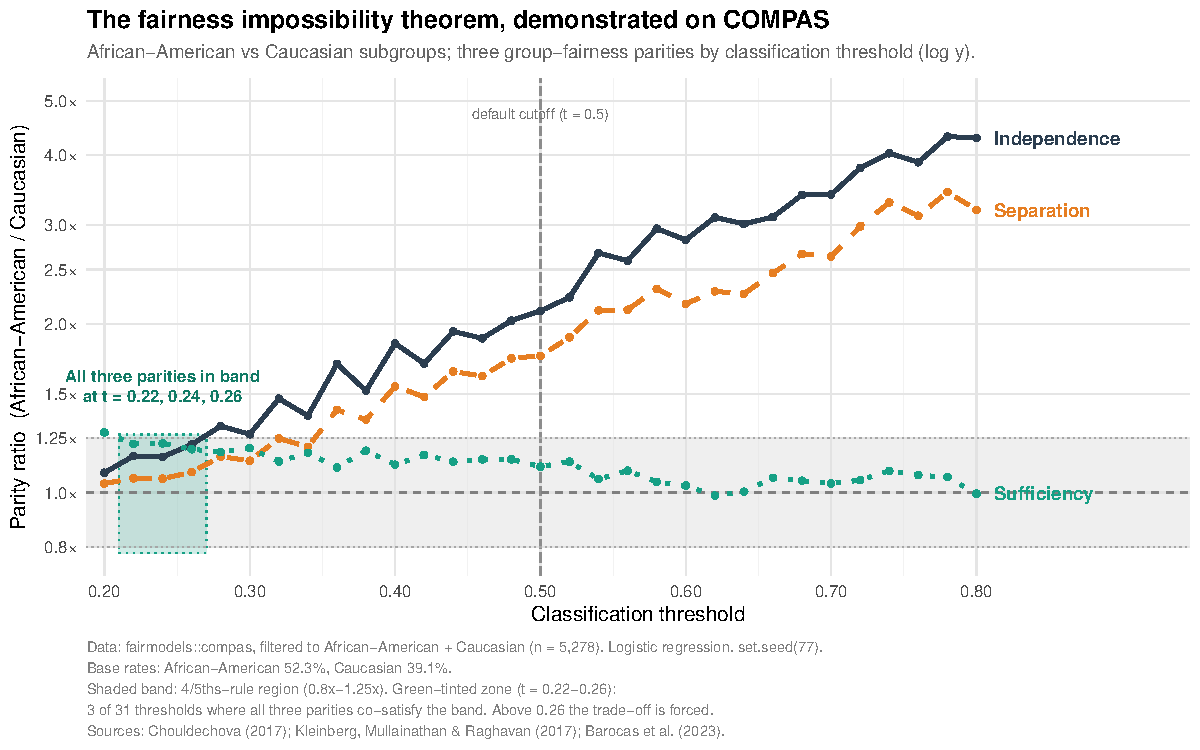
\includegraphics[width=\linewidth]{fig3_impossibility_demo.pdf}
  \caption{Empirical demonstration of the Chouldechova--Kleinberg-Mullainathan-Raghavan impossibility theorem on the COMPAS dataset. Replication procedure: the COMPAS dataset bundled with the \texttt{fairmodels} R package \citep{wisniewski2022} (originally released by ProPublica, \citealp{angwin2016}), filtered to the African-American and Caucasian subgroups ($n = 5{,}278$); a single logistic regression of two-year recidivism on number of prior offences, age band, misdemeanour status, sex, and ethnicity; seed 77; the Independence, Separation and Sufficiency parity ratios computed across a threshold grid 0.20--0.80 in steps of 0.02 (31 thresholds). Shaded band: the 4/5ths-rule region (0.8--1.25). The three parities trace incompatible trajectories.}
  \label{fig:impossibility}
\end{figure}

The implication for Article~10 is direct, and \citet{wachter2021} draw the bridge explicitly: the impossibility theorem complicates the relationship between EU non-discrimination law and bias-mitigation engineering. EU law treats discrimination as a relational violation between protected groups. The impossibility theorem treats fairness as a property of a classifier with respect to a population. When base rates diverge, as they do for hiring outcomes between the majority and MENA-origin minorities (Section~\ref{sec:external}), the relational equality EU law requires cannot be reached by a classifier without sacrificing one of the three desiderata. Article~10 tells deployers to \enquote{detect, prevent and mitigate possible biases} but cannot tell them \emph{which} fairness criterion to satisfy, because the choice is not technical. Sufficiency says the score means the same thing across groups. Separation says errors fall evenly across groups. Independence says representation matters more than error. The choice among them is political, and each excludes the others. The result also presupposes group-statistical operationalisation; counterfactual approaches \citep{kusner2017} avoid the trichotomy but face causal-identification difficulties the AI Act's procedural language ignores.

Article~14's human-oversight mechanism inherits the impossibility instead of resolving it. The overseer is supposed to step in when the system errs. But the trade-off they would be stepping into has no technical solution: it is the political choice among Sufficiency, Separation, and Independence that no classifier can take. Article~14 hands that choice to a designated natural person, usually an employee of the deployer, rather than to an institution accountable for the underlying constitutional question. A substantive decision moves out of public reason and into operational discretion.

The structural upshot: the AI Act's bias-mitigation regime rests on a presupposition that its own mathematics disproves, and disproves precisely for the populations the regime most needs to protect. Statistical fairness is not the engineering target it is treated as.

Before turning to the external evidence, one connection deserves a name. The internal and external failures share one gesture: the reduction of fairness to a property of a population, captured by statistical equality. The gesture operates on two distinct senses of \enquote{population}, a classifier-input distribution on one side and the polity-member set produced by recognition on the other, and collapses them. The internal failure shows the gesture cannot succeed even when the classifier-input population is given; the external failure shows the gesture takes the polity-member population for granted, presupposing the polity that produced the data and made equality among its members substantively possible. Two faces of one operationalisation error: \citet{wachter2021} name the internal expression, \citet{arendt1951} the external.

% =====================================================================
\sectiontwo{The External Failure}{Audit Evidence and the Polity's Prior Exclusion}\label{sec:external}
% =====================================================================

Where the impossibility result establishes that the AI Act's bias-mitigation regime cannot internally fulfil its own remit, the audit-study evidence shows that the populations the regime most needs to protect are those for whom the divergence of base rates is empirically severe and rising. Figure~\ref{fig:forest} synthesises seven cross-national audit studies of name-based hiring discrimination (2004--2023); the 2024 LLM-side audit by \citet{wilsoncaliskan2024} uses a different metric and is treated separately below.

\begin{figure}[h]
  \centering
  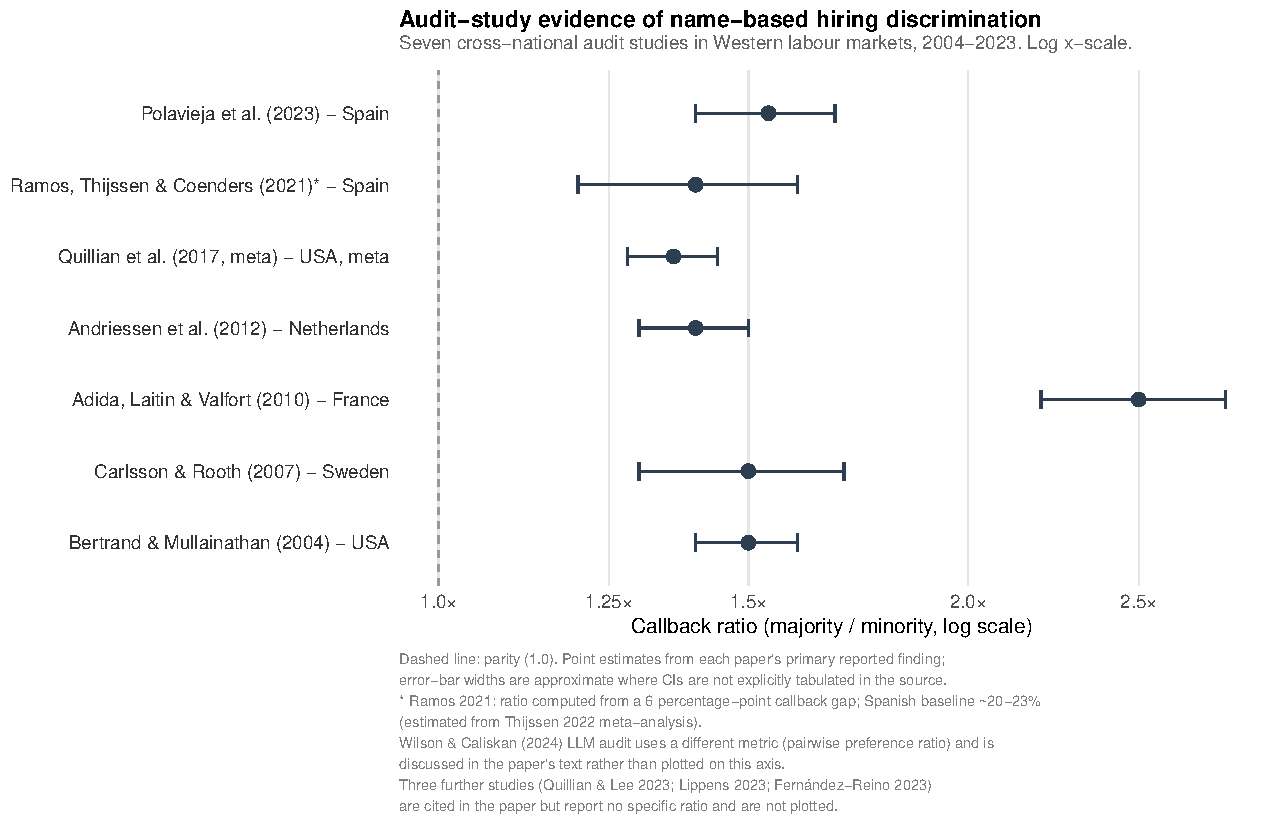
\includegraphics[width=\linewidth]{fig1_forest_plot.pdf}
  \caption{Effect sizes from seven cross-national audit studies of name-based hiring discrimination in Western labour markets, 2004--2023. Callback ratio of majority over minority on a log scale; vertical dashed line at parity (1.0). The Ramos~et~al.~(2021) ratio is computed from a six-percentage-point callback gap; the Wilson \& Caliskan~(2024) LLM audit uses a non-comparable preference-ratio metric and is reported in the body of Section~\ref{sec:external} rather than plotted here.}
  \label{fig:forest}
\end{figure}

The canonical baseline is \citet{bertrandmullainathan2004}: White-named applicants in Boston and Chicago received fifty per cent more callbacks than equivalently-credentialled Black-named applicants. \citet{carlsson2007} report a comparable gap for Arabic-named men in Sweden; \citet{adida2010} find Muslim Senegalese applicants in France 2.5 times less likely than Christian Senegalese counterparts, holding country-of-origin constant. The Spain-specific data point from \citet{ramos2021} documents a six-percentage-point callback gap for Moroccan applicants, consistent across regions and not driven by unemployment.\footnote{The Figure~\ref{fig:forest} ratio of 1.40 is computed from this six-percentage-point gap, assuming a Spanish-named callback baseline of approximately 20--23\%, consistent with the \citet{thijssen2022} meta-analysis of 94 Western field experiments; the ratio is robust to baseline assumptions within the 18--25\% range.}

\citet{fernandezreino2023} complicate the picture: veiled Muslim women in Spain face substantially \emph{less} discrimination than counterparts in Germany or the Netherlands, a finding any European-wide framing must survive. The heterogeneity is a refinement, not a refutation: different polities exclude differently, in country-specific patterns the paper does not adjudicate. That is consistent with the Arendtian frame developed here, which makes the polity (not Europe) the unit of analysis. The aggregate trend remains directional. \citet{quillian2023} aggregate ninety field experiments across six countries to show that hiring discrimination against MENA-origin applicants \emph{increased} during the 2000s, the only major demographic for whom discrimination is rising. \citet{lippens2023} confirm in the most recent meta-analysis that ethnic hiring discrimination shows no structural decline. This is the empirical baseline against which Article~10 must operate.

The transition from human to algorithmic gatekeeping does not correct the picture. \citet{wilsoncaliskan2024} test three open large language models on more than three million pairwise resume comparisons across nine occupations: White-associated names are preferred 85.1 per cent of the time over Black-associated names, and Black male names are preferred over White male names in 0 per cent of pairwise comparisons, a degenerate distribution no group-statistical mitigation can correct without altering the substrate that produced it. The result is the LLM-side analogue of \citet{bertrandmullainathan2004} at the scale of automated resume-screening pipelines, the very systems Annex III, point 4 of the AI Act classifies as high-risk.

\begin{figure}[h]
  \centering
  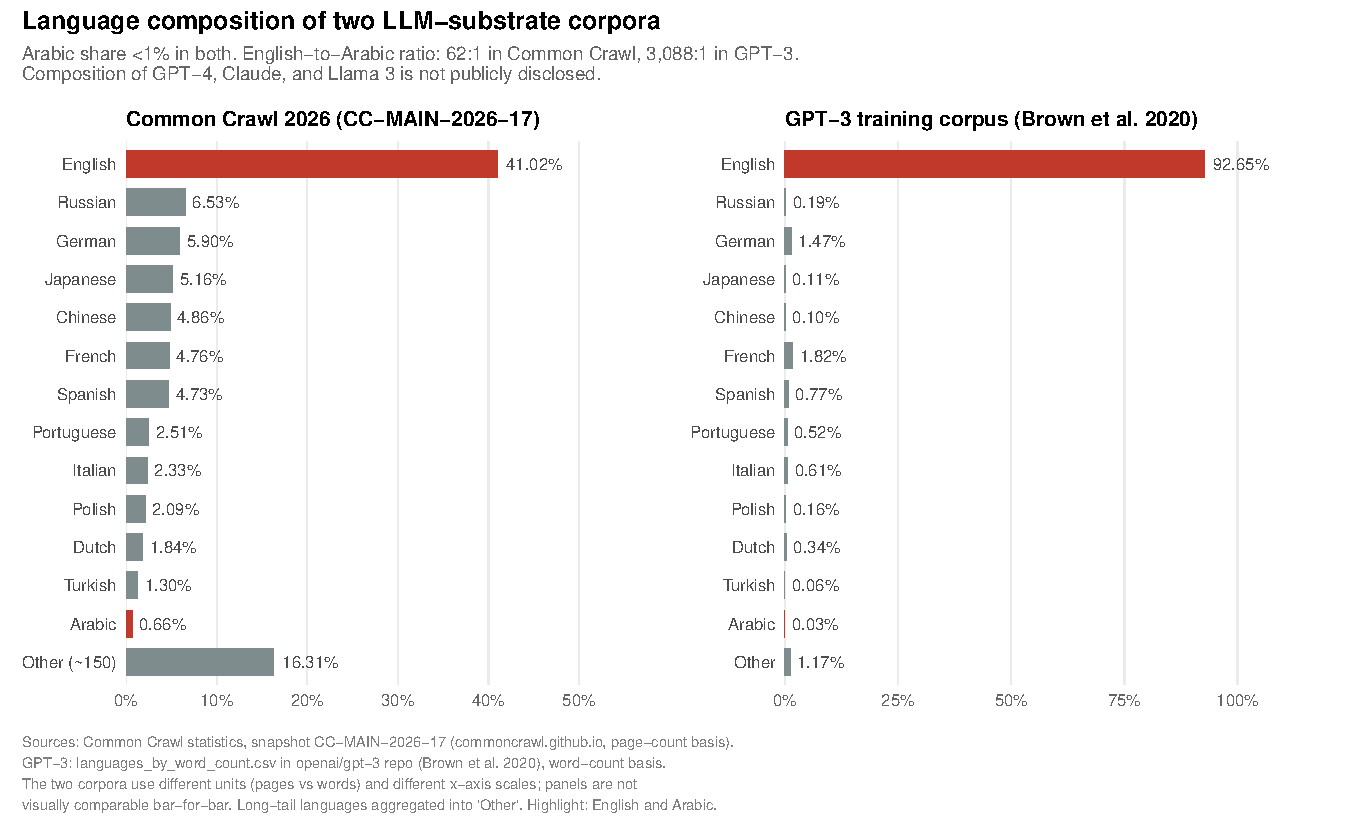
\includegraphics[width=\linewidth]{fig2_language_composition.pdf}
  \caption{Language composition of two LLM-substrate corpora. Common Crawl 2026 (left, snapshot CC-MAIN-2026-17; \citealp{commoncrawl2026}) and the GPT-3 training corpus (right, \citealp{brown2020}) are both predominantly English (41\% and 93\% respectively); Arabic share is below one per cent in both. The training-data composition of GPT-4, Claude 3.5, and Llama 3 has not been publicly disclosed by their developers.}
  \label{fig:fig2}
\end{figure}

The substrate compounds the problem. Figure~\ref{fig:fig2} shows that 41 per cent of Common Crawl 2026 is English and 0.66 per cent is Arabic; the GPT-3 training corpus \citep{brown2020} is 93 per cent English. Cultural-alignment audits of frontier models against the World Values Survey across 107 countries find Jordan and Libya among the most distant from GPT-4o's revealed values \citep{tao2024}. \citet{zuboff2019} reads such corpora as the artefact of a political economy that pre-decides whose voices the substrate carries. The substrate finding bites directly on Article~10, which requires training data to be \enquote{relevant, sufficiently representative, and to the best extent possible, free of errors and complete}: for downstream high-risk systems trained on these corpora, the representativeness requirement is empirically defeated before any specific deployer chooses, and the AI Act does not regulate the substrate \citep{vealeborgesius2021}. The populations whose hiring outcomes the AI Act most needs to protect are the populations for whom the LLM substrate is least prepared.

The polity that generated both the audit record and the LLM corpus has already constituted these populations as marginal in labour-market access and substrate representation; Arendt names the polity-level analogue. Bias-mitigation cannot repair what the polity has not yet decided to repair.

% =====================================================================
\sectiontwo{Three Vignettes}{The Phenomenology of Polity-Loss}\label{sec:vignettes}
% =====================================================================

The autoethnographic strand is licensed by \citet{ellis2011} and follows \citet{costanzachock2018}, who opens an MIT \emph{Journal of Design and Science} essay on AI ethics with their own experience of TSA millimeter-wave scanners. The three vignettes that follow do not generate the argument; they triangulate it, illustrating from the inside what the literature records at scale.

\textit{Vignette 1.} What changed my application strategy was less the data than the texture of the silence: replies arrived slowly or not at all to applications I was credentialled for (a bachelor's from this university and a master's in progress, professional experience, four working languages), while Spanish-named acquaintances with comparable credentials reported the opposite rhythm. Audit-study literature \citep{ramos2021,quillian2023,wilsoncaliskan2024} records the structural pattern at scale.

\textit{Vignette 2.} I left Damascus at fourteen, the year the city's eastern districts began to be called by different names by different broadcasters. My emotional vocabulary in Arabic stopped developing then. \citet{pavlenko2014} documents this displacement among multilingual speakers. Figure~\ref{fig:fig2} shows the corpus substrate of the AI systems that meet me in those languages.

\textit{Vignette 3.} When I am with Syrian friends in Madrid, I am too European. Too willing to ask direct questions, too quick to press the implicit toward the explicit, too convinced that one's name is one's own to negotiate. When I am with Spanish or other European colleagues, I am the Middle Eastern friend, my standpoint flagged not by anything I say but by where my voice is presumed to come from. This double-positioning is the socio-cultural analogue of what Arendt diagnosed politically: the loss of \enquote{a place in the world which makes opinions significant and actions effective} \citep[p.~296]{arendt1951}. The two are not identical: Arendt's stateless lost jurisdiction; the double-positioned migrant retains it. What is lost is the unmarked standing that lets ordinary speech do its ordinary work. The words that sort us, \emph{expat} or \emph{immigrant}, settle that unmarked standing before I speak \citep{kunz2020}.

% =====================================================================
\sectiontwo{The Killer Move}{Article 111 and the Statelessness Exemption}\label{sec:art111}
% =====================================================================

The audit evidence and the vignettes show the polity withholding recognition before any law acts. The strongest evidence that the AI Act encodes that withholding is in its own transition rules. Article~111 of Regulation 2024/1689 \citep{aiact2024} sets out how the regulation applies to AI systems already on the EU market when most of it enters into force on 2~August 2026. Its central provision concerns Annex~X, which lists the European Union's large-scale IT systems for external borders and the management of asylum, migration, and visa applications: the Schengen Information System, the Visa Information System, Eurodac, the Entry/Exit System, ETIAS, ECRIS-TCN, and the interoperability framework that ties these databases together. For AI components in these systems, full enforcement is deferred until 31~December 2030, more than four years after the rest of the regulation begins to apply.

The deferral is not incidental. It is a deliberate concession to the operational complexity of retrofitting border-management infrastructure to high-risk obligations. Each Annex~X system is a multi-Member-State, multi-vendor, multi-decade engineering programme; trying to amend them all at the same time would be administratively unrealistic. From a public-administration perspective the rationale is reasonable. Administrative feasibility and political priority, however, are not separable here: feasibility constraints are accepted as binding only for populations the polity already treats as deferrable. From an Arendtian perspective the deferral is the diagnosis itself.

The Annex~X systems are not abstract instances of the high-risk category listed in Annex III, point 7. They are where the migrant actually meets the EU polity: the asylum claim recorded at Eurodac, the visa decision rendered at the VIS, the entry permission determined at the EES, the no-fly classification assigned at ETIAS. They are the points at which a person's right to enter, to claim refuge, to be recognised as a member of any community is decided by automated means. That this category, and only this category, has its enforcement deferred for four extra years is not a regulatory accident. The AI Act is acknowledging, in its own text, that the populations it most struggles to extend rights to are the ones at the polity's edge.

In Arendt's language, this is a deferral of the right to have rights. The bias-mitigation regime built by Articles 10, 14, 27, and 86 does not yet apply to the systems through which the polity decides who counts. Article~111 makes that deferral textual.

Before closing, two charges against the autoethnographic strand: that the vignettes read as memoir, and that n=1 first-person evidence is vulnerable to selection and recall bias. The vignettes are not evidence for the audit-study pattern; Figure~\ref{fig:forest} does that work. They are evidence for what that pattern feels like from inside the polity that produces it, which is the register Arendt's diagnosis lives in.

% =====================================================================
\sectiontwo{Conclusion}{Equality Cannot Be Optimised}\label{sec:conclusion}
% =====================================================================

Two parallel failures structure the argument. The first is internal: when subgroup base rates differ, no classifier can jointly satisfy independence, separation, and sufficiency \citep{chouldechova2017,kleinberg2017,barocas2023}. Article~10's mandate to detect and mitigate biases cannot be operationalised without a political-philosophical choice among incompatible fairness criteria. The second is external: the populations whose hiring outcomes audit-study evidence has tracked across two decades \citep{quillian2023,ramos2021,wilsoncaliskan2024} are those for whom the polity producing the data has already withheld substantive equality. Article~111's deferral of large-scale migration-AI enforcement until 2030 textualises this withholding.

The two failures are not the same failure. They are homologous failures of one universalist gesture: that political fairness can be operationalised as the equality of group-statistical metrics. The gesture fails on its own internal terms because the mathematics rules it out, and on its external terms because Arendt has named a precondition, the polity that constitutes substantive equality, that no statistical apparatus can produce.

Three limitations frame this argument's reach. First, the audit-study synthesis in Figure~\ref{fig:forest} is descriptive: it visualises effect sizes across studies but does not estimate a formal meta-analytic model with heterogeneity diagnostics, which a follow-up paper could supply. Second, the empirical evidence is restricted to Western labour markets and a single US criminal-justice dataset; the polity-precondition argument may transpose to non-Western regimes but is not tested here. Third, the autoethnographic strand, even properly licensed, illustrates rather than proves.

What does this leave the AI Act? Not nothing: transparency obligations, a right to explanation, the FRIA, the Recital~48 list of Charter rights are accomplishments, and an advance over the unregulated status quo. The architecture cannot supply a polity it presupposes. What it can do is acknowledge its own limits and refer the political question back, via Article~112's mandatory evaluation cycle, to the legislative institutions whose work no statistical apparatus can replace.

\begin{quote}
\noindent
We are not born equal; we become equal as members of a group on the strength of our decision to guarantee ourselves mutually equal rights \citep[p.~301]{arendt1951}.
\end{quote}

\noindent Equality is not a quantity to be optimised. It is a polity to be constituted.

% =====================================================================
\bibliography{references}
% =====================================================================

\end{document}
